\documentclass[SE,authoryear,toc]{lsstdoc}
% lsstdoc documentation: https://lsst-texmf.lsst.io/lsstdoc.html
\input{meta}

% Package imports go here.
\usepackage{graphicx}

% Local commands go here.

%If you want glossaries
%\input{aglossary.tex}
%\makeglossaries

\title{Aux Tel Tracking Problem Report Nov 2021}

% Optional subtitle
% \setDocSubtitle{A subtitle}

\author{%
Christopher Stubbs
}

\setDocRef{SITCOMTN-022}
\setDocUpstreamLocation{\url{https://github.com/lsst-sitcom/sitcomtn-022}}

\date{\vcsDate}

% Optional: name of the document's curator
% \setDocCurator{The Curator of this Document}

\setDocAbstract{%
This note describes an Aux Tel tracking jump detected nights of Nov 2-5 2021
}

% Change history defined here.
% Order: oldest first.
% Fields: VERSION, DATE, DESCRIPTION, OWNER NAME.
% See LPM-51 for version number policy.
\setDocChangeRecord{%
  \addtohist{1}{YYYY-MM-DD}{Unreleased.}{Christopher Stubbs}
}


\begin{document}

% Create the title page.
\maketitle
% Frequently for a technote we do not want a title page  uncomment this to remove the title page and changelog.
% use \mkshorttitle to remove the extra pages

% ADD CONTENT HERE
% You can also use the \input command to include several content files.


\section{Introduction}

On the night of 2021-11-03 there were multiple instances of sudden jumps in Aux Tel telescope boresight pointing, in the midst of a collection of sequential images. The magnitude of the pointing jumps is 3--5  arcseconds. 

This merits attention by the Aux Tel telescope engineering team. It's unclear at present whether this is originating in the Alt-Az-Rotator system or the lookup table for the secondary hexapod. 

\section{Images and Analysis}

Table \ref{tab:table} shows the date, sequence numbers, centroids, and offsets for the images in question. Exposure times The intermediate images, 656 and 665, show dual stellar images and caught the problem as it occurred. Figures \ref{fig:image} and \ref{fig:imagezoom} show frame 656 that has the dual-PSF symptom clearly evident. 

\begin{table}[]
    \centering
    \begin{tabular}{|l|l|l|l|l|l|l|}
    \hline
    date & seq nums & X1 & Y1 & X2 & Y2 & dr (pixels) \\
    \hline
    20211103     & 655, 657 & 2079.6 & 1328.4 & 2128.5 & 1311.1 & 51.9\\
    20211103     & 664, 666 & 1855.0 & 1714.4 & 1885.4 & 1701.4 & 33.0 \\
    \hline
    \end{tabular}
    \caption{Images and corresponding centroids and offsets in Aux Tel boresight. }
    \label{tab:table}
\end{table}

\begin{figure}
    \centering
    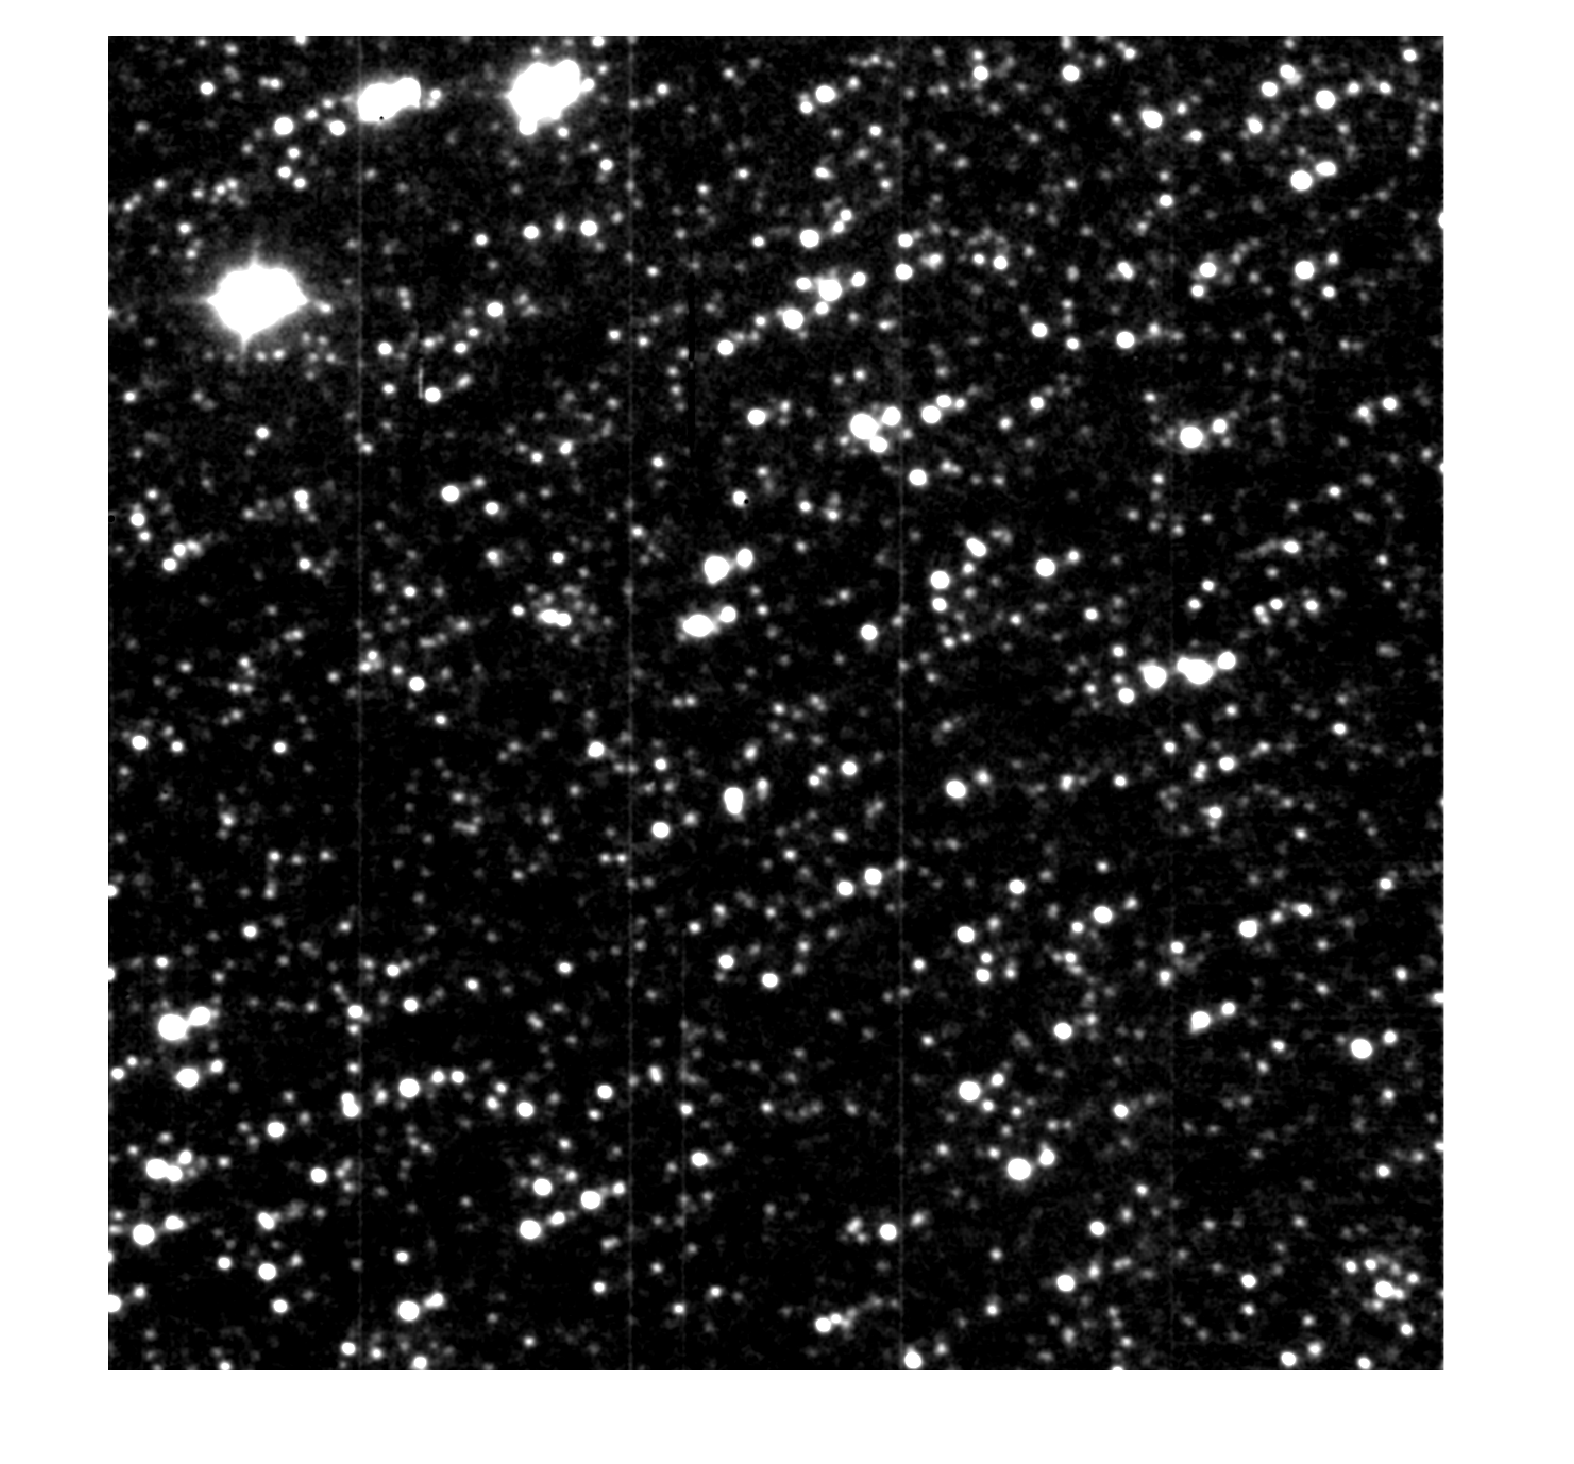
\includegraphics[width=6in]{Image656png.png}
    \caption{Image 656.}
    \label{fig:image}
\end{figure}

\begin{figure}
    \centering
    \includegraphics[width=6in]{Image656zoom.png}
    \caption{Image 656 zoom. Each PSF has a fainter replica located up and to the right, due to boresight shift during the exposure.}
    \label{fig:imagezoom}
\end{figure}

\section{Tentative Diagnosis and Recommendations}

Something is causing sudden offsets in Aux Tel pointing. We suggest looking at EFD data on the drive and hexapod motions for images 656 and 665 on 20211103. Determining the direction of the offset in telescope mount coordinates (Alt, Az) would also be informative. 

\appendix
% Include all the relevant bib files.
% https://lsst-texmf.lsst.io/lsstdoc.html#bibliographies
\section{References} \label{sec:bib}
\renewcommand{\refname}{} % Suppress default Bibliography section
\bibliography{local,lsst,lsst-dm,refs_ads,refs,books}

% Make sure lsst-texmf/bin/generateAcronyms.py is in your path
\section{Acronyms} \label{sec:acronyms}
\input{acronyms.tex}
% If you want glossary uncomment below -- comment out the two lines above
%\printglossaries





\end{document}


